\chapter{はじめに}
\label{introduction}

\section{研究背景}
\label{subject}
``Embodiment''という言葉が、心理学やロボティクス、バーチャルリアリティ(VR)、ヒューマンインターフェースデザインなど、さまざまな分野で注目されている。Botvinick \& Cohenによるラバーハンド錯覚\cite{BotvinickCohen1998}の報告は、私たちが自分の身体として認知する対象は生まれ持った肉体に限らないことを示した。それを皮切りに、「私たちはどこまでを自分の身体として認識しうるか?」、すなわち「何を``身体化''できるのか?」について、その可能性と限界を探る研究が次々と発表されている。また、インターフェース研究者の渡邊は「まさに自分自身の身体である」という感覚を指すGallagherの``sense of ownership''を「自己帰属感」と訳し、インターフェースにおける直感操作を実現する重要な指針として、「身体化」の議論との橋渡しをした。Embodimentの訳は「身体化、一体化、身体性」など文脈によって異なるが、これらについては「身体化」と訳すことが適当だと思われる。そして、「``身体化''としてのembodiment」は、人間の可能性の拡張や、直感的で便利なインターフェースを実現するためのデザインへの応用へと広がっている。

% インターフェース研究者の渡邊は、インターフェース設計における理想形を「透明化」であると説明する\cite{Watanabe2017}。すなわち、どんなに複雑で高度な道具であっても、原始的な道具のように原因と結果の関係が直接的であり、道具そのものに対して意識することなくそれを使用できることこそが理想とした。

% そして渡邊は、その理想を実現するための重要な指針が「自己帰属感(sense of ownership)」であると提言する。自己帰属感とは、「あたかもその装置が身体の延長であるかのように感じられる」感覚を指す。

% 人々を取り巻くものが機械や情報処理によって高度化する中、人々と機械との接点を設計することが重要となった。
% ここで、人々と機械との最適な関係を「より使いやすく有用に」\footnote{国際標準化機構(ISO)による「人間中心設計」の導入部\cite{hcd}より}することとし、それを具現化してきたのがエルゴノミクス、人間中心設計といった設計論である。

% 道具の使用における行為と結果の関係から捉えたとき、「使いやすさ」とは、原始的な道具のように直接的であり、道具そのもに対する意識がなくなっていく「透明化」を指す。

% 渡邊は、その理想を実現する指針として「自己帰属感」という概念を導入し、例えばマウスカーソルやスマートフォンのような「操作時の指とグラフィックの追従性が高い」インターフェースは自身の一部や延長として感じられる、「透明」なインターフェースであると説明する。

% こうした設計論は、確かに複雑で高度な道具の力を借りて人間の活動の可能性を拡げることに貢献してきた。
しかし、これらの議論だけでは、embodimentについて見落とされている側面があるのではないだろうか。上記でみてきたembodimentは、「私たちの身体に帰属する他者」という関係性だった。ここではその逆の、「他者に帰属する私たち」という関係性について考えてみたい。例えばそれは、ピアノと人との間に生起する。ピアノを初めて弾くとき、奏者は手の大きさによる制約を受け、最初のうちは左右別々に指を動かすだけでも困難さを経験する。しかし、試行錯誤を経て、ピアノの制約と自身の身体能力との間で折り合いをつけていくことで、ようやく楽器を通して表現ができるようになる。ミュージシャンのスキャットマン・ジョン(ジョン・ポール・ラーキン)は、「吃音症」という発話障害を抱え、「自身の身体」という切っても切り離せない存在をコントロールできない中、むしろその症状を逆手に取るように「テクノスキャット」という独自の歌唱法を開拓した。こうした方法をとって他者と調和していくことは、上記の議論とは逆向きのembodimentと言えるのではないだろうか。

こうした関係について考えるにあたっては、embodimentを「自己」と「他者」の関係に対して中立的な``一体化''と訳すことが適当だと考える。そして、「自己」と「他者」のあいだで相互に折り合いをつけていくようなこの``一体化''は、そうなるまでの過程における困難と、それを克服してうまいやり方を見出していく、高度な人間性の発揮による喜びと、創造性を内在している。

そこで本研究では、「自己」と「他者」の双方向的な一体感が象徴的に現れる「人馬一体」という言葉に注目した。この一体化のプロセスは、例えば楽器やバイクなどにもみられる。これを具現化するような関係性が芽生える体験は、いかにして設計できるのか。この問いについて、手指の変換表現からアプローチしていく。

% \section{リサーチクエスチョン}
% \label{research_question}
% 前節では、研究背景に触れ、本研究が「人馬一体」と言われるような、相互の折り合いをつけながら生まれる親密さについて探索するものであると説明した。ここでは、探索の上での中心的な問いについて明記する。

% \begin{quote}
% \textbf{対象からの影響も受けつつ、相互の折り合いをつけながら生まれる一体感はどのように生まれるのか。そして、それはいかに設計できるのか。}(最後に回収)
% \end{quote}

% 本研究では、「手指とは異なる形状への変換」を通して「身体の中の他者性」を経験させる表現を探索することからこの問いに迫った。

\section{研究概要}
本研究では、手指とは異なる形状への変換から「身体の中の他者性」を経験させる表現によって、人馬一体のような「一体感」の生起を目指した。探索的におこなったプロトタイピングについて、「``一体化''としてのembodiment」から、人と対象との関係を分類したとみられるコンピュータ工学者Sydney Felsの提唱する概念を用いて分析した。その上で、重要だと考えられる表現で構成された修士作品《Grasp(er)》を制作した。本研究の狙いは、この作品の制作と体験の分析を通して「人馬一体感」を経験するデザインの道筋を示すことである。「人馬一体感」が実現しているかについては、4名の作品体験を振り返ることから考察する。

\section{「身体の中の他者性」に取り組む動機}
\label{prototyping_concept_making}
本研究は、「人馬一体感」の生起に、手指とは異なる形状への変換から「身体の中の他者性」を経験させる表現を通して探索する。この表現から取り組むこととした動機は、この表現を取り組むこととした動機は、「動きのスケッチツール」という目的で制作した習作「Digitize」の展示が関係している。この展示で、たまたま目に止まった体験者の様子が、 \ref{subject}節で述べた問題意識の切り口に繋がると捉えた。
この節では、その習作について説明し、この表現を通して「人馬一体感」を探索することの動機とする。

習作「Digitize」とは、手指の動きを別の形へとマッピングさせた3つの変換表現から構成された作品である。静止画について構想を膨らませる際、「紙とペン」を通して直接イメージをスケッチできるが、動きについてもそれに相当するほど、直感的かつ、高い表現力でスケッチができるツールを作ろうとした。そこで、動きに対して高い表現力を有する手指を使って、「動きをスケッチする」ツールを案じていた。しかし手指の動きをそのまま表示するのでは、手指を使うことの意義が薄い。手指は人間の身体の中でも高い表現力をもつ器官である。もし「手ではない形」を通してでも、様々な形や動きを自由に作れるのなら、人間の身体構造による制約を超えた「動きのスケッチ」ができ、手指を使うことの意義があるのではないかと構想した。
そうして、手指の動きをトラッキングするが、画面上では別の形へマッピングされて動くインターフェースについて、プロトタイピングを行った。そのプロトタイピングは、2022 年 7 月に岐阜県大垣市で開催されたイベント「IAMASOpen House 2022」にて展示した\footnote{\url{https://k1105.github.io/eee_openhouse_2022/}}。この時点では、動きを記録する機能は存在しておらず、あくまで、手指とは異なる形状が手の動きに伴って動くのを確認するだけのものであった。

\begin{figure}[H]
  \centering
  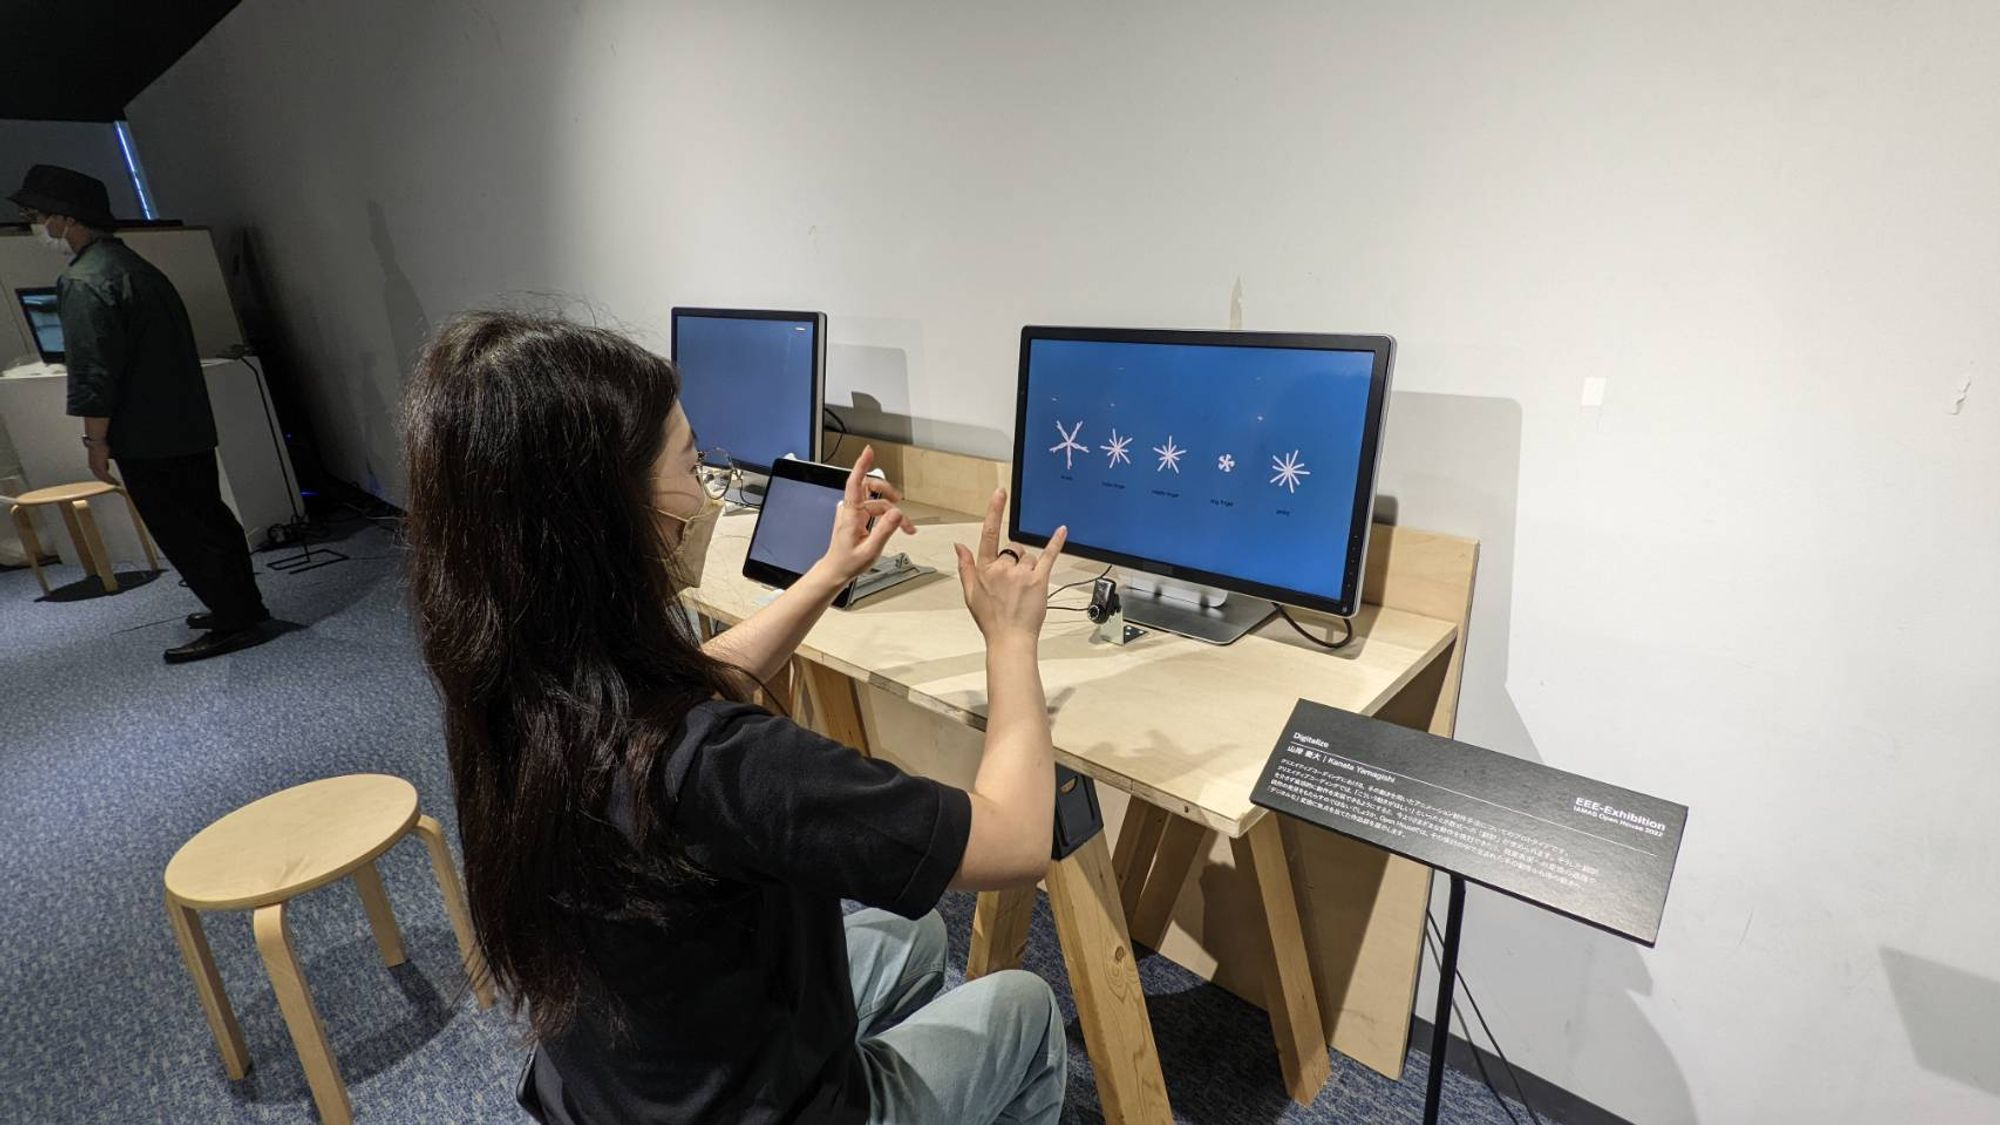
\includegraphics[width=15cm]{img/openhouse2022.jpeg}
  \caption{IAMAS Open House 2022での展示の様子(2022年)}
  \label{fig:exhibit_2022}
\end{figure}

\begin{figure}[H]
  \centering
  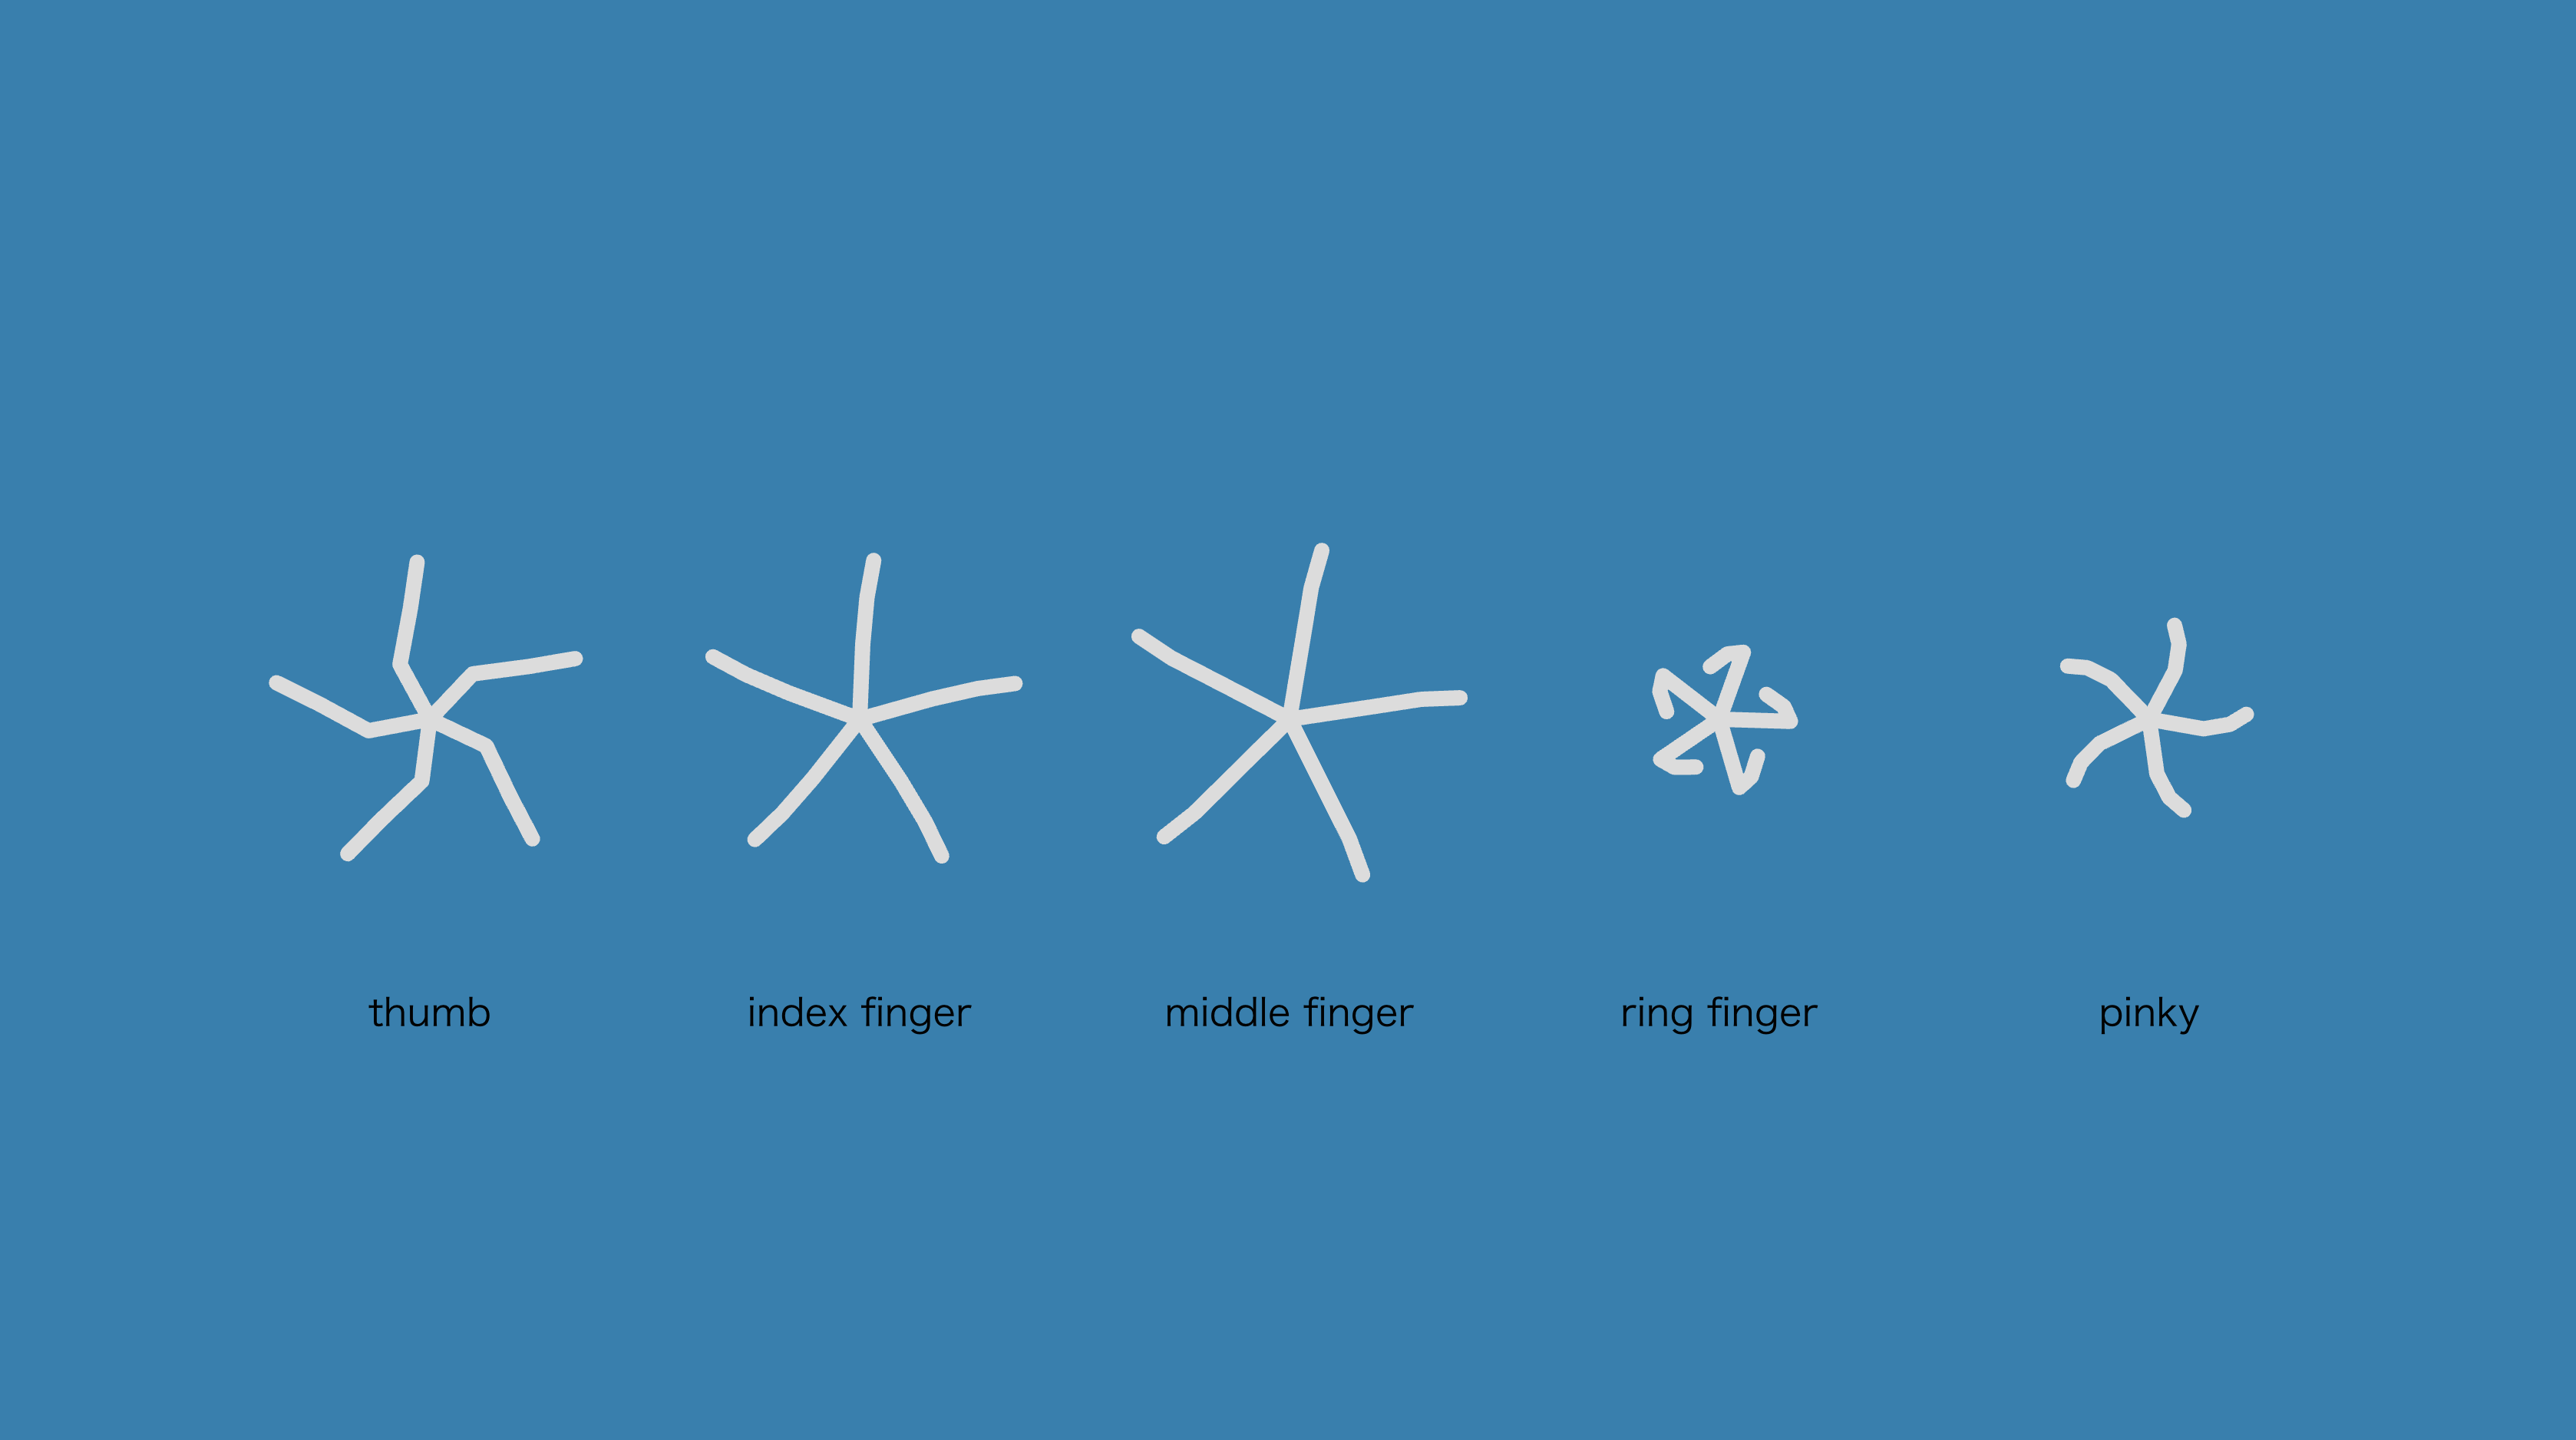
\includegraphics[width=15cm]{img/openhouse2022_interface.png}
  \caption{Digitizeのインターフェース(2022年)}
  \label{fig:exhibit_2022_interface}
\end{figure}

しかし展示を行うと、想定していなかった習作の魅力に気づいた。それは、指の動きが単に、別の構造にマッピングされただけであるのに、別の構造の手を動かす体験はそれだけで興味を惹くものだということである。手指とは異なる形状への変換が3パターン展示された状態のこの展示で、10分以上興味を持って体験する方が複数名いた。そして、仕組みとしては指先と付け根の距離をとっているのだが、その変換処理を「正しく」理解していなくても、異なる方法で理解しているように思われる人が何人かいた。指先と付け根の距離を評価して変換していても、カメラに対して手を近づけたり遠ざけたり、手首から傾けたりすることでも動かすことはできる。そのためか、さまざまな「わかり方」があったのだと考えた。仕組みを知っている制作者にとっては自明なことだが、自己の運動とどう対応するのかを知り得ない体験者は、自身の体を動かして観察されたことを通して推測することになる。それゆえに、この仕組みを通して思い描く身体像に、体験者ごとに違いがあるのではないか。

こうした体験者ごとの違いは、「わかりやすい」ものを対象としたときよりも、「わかりにくい」ものを対象としたときの方が顕著に現れると考えた。その上で、わかったようで分からない、行きつ戻りつな感覚に陥りながらも、飽きずにそれを分かろうとして向き合う様子が続いたことに、先の問題意識に応えるものがあるのではないかと考えた。

\section{本研究の目的}

本研究の目的は、人と道具、機械、あるいは人体の中にある他者性との関係における「人馬一体」のような一体感について捉えることである。そして、そうした関係性はどのようにして引き出すことができるのかを提示することである。

\section{本論文の構成}
(提出前に、全文章を概観した上で書き直す)

本章では、研究背景を問題提起の形で示し、研究の概要を示した。本研究が着目した「手指とは異なる形状への変換」について、その観点から取り組む動機と、

第\ref{related_works}章では、「身体化」に関する先行研究について、それぞれの分野でどのように展開しているのかについてを概観する。そして、その中での本研究の位置付けと貢献を示す。

第\ref{prototyping}章では、手指の変換表現についての探索と、「人馬一体感」の生起に向けた意識的な試行が生じる体験として作品を構成するにあたっての取捨選択のプロセスを説明し、最終的な作品における構成の根拠を示す。

第\ref{about_grasper}章では、作品概要と、そこに至るまでのプロトタイピングの分析を通して、作品形態について説明する。

第\ref{validation}章では、そのようなねらいのもと制作された本作品が、実際どのように経験されるのかについての質的調査を行うため、Video Cued Recallという手法を用いて体験について振り返り、実際の体験がどのようなものであったのかを踏まえて、モデルとの関係性について考察する。

第\ref{考察}章では、行った調査の結果からどのような体験の作品であったかを振り返り、本作品が狙いとしていたこと、あるいはその範疇を超えて、作品として何が達成されたのかについて考察する。

第\ref{matome}章では、これまでの議論をまとめ、最後に今後の展望として、ここで制作を行ったモデルがそれ以外の議論とどのように関係し、今後どのような可能性を有するのかについて述べる。